\documentclass[10pt]{article}
\usepackage[polish]{babel}
\usepackage[utf8]{inputenc}
\usepackage[T1]{fontenc}
\usepackage{amsmath}
\usepackage{amsfonts}
\usepackage{amssymb}
\usepackage[version=4]{mhchem}
\usepackage{stmaryrd}
\usepackage{graphicx}
\usepackage[export]{adjustbox}
\graphicspath{ {./images/} }

\title{Zadania - etap I (szkoła podstawowa) }

\author{Oświadczenie\\
Niniejszym oświadczam, że jako uczestnik konkursu „OD SZKOLNIAKA DO ŻAKA" zorganizowanego przez Centrum Nauczania Matematyki i Kształcenia na Odległość Politechniki Gdańskiej, wyrażam zgodę na przetwarzanie moich danych osobowych w zakresie niezbędnym dla potrzeb niniejszego konkursu.\\
Przyjmuję do wiadomości, że moje dane osobowe będą wykorzystane zgodnie z ustawą z dnia 29 sierpnia 1997 r. o ochronie danych osobowych (Dz.U. z 2002 r. nr 101, poz. 926 ze zm.) dla celów przeprowadzenia w/w konkursu.\\
Jednocześnie oświadczam, że zostałem poinformowany o tym, że:\\
- Administratorem danych osobowych konkursu jest: Politechnika Gdańska z siedzibą przy ul. Gabriela Narutowicza 11/12; 80-233 Gdańsk\\
- Przysługuje mi prawo do wglądu do moich danych i żądania ich poprawienia.\\
- Dane będą przetwarzane dla realizacji konkursu.\\
- Podanie danych jest dobrowolne.\\
- Nie przewiduje się przekazywania danych.}
\date{}


\begin{document}
\maketitle
Zadanie 1. Jeżeli do pewnego ułamka dodamy jego trzecią część oraz jego piątą część, to otrzymamy 1. Jaki to ułamek?

Zadanie 2. Dany jest kwadrat KLMN, którego pole wynosi \(36 \mathrm{~cm}^{2}\). Punkty A, B, C, D leżą na bokach kwadratu KLMN oraz długości odcinków KA, LB, MC i ND są jednakowe i wynoszą 1cm. Oblicz pole czworokąta ABCD.\\
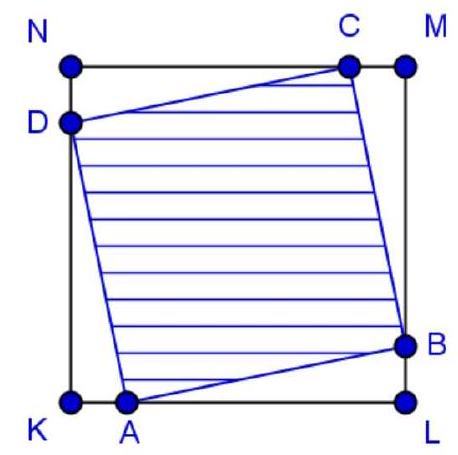
\includegraphics[max width=\textwidth, center]{2024_11_21_dcd2fc8702c4ba725104g-1(1)}

Zadanie 3. Średnia wieku grupy 9 dziewcząt wynosi 15 lat. Uwzględniając instruktorkę tej grupy, średnia wzrosła do 16 lat. lle lat ma instruktorka?

Zadanie 4. Dane są kwadrat ABCD i trójkąt równoboczny KLM (patrz poniższy rysunek). Wiemy, że kąt \(\alpha\) ma miarę \(50^{\circ}\). Oblicz miary kątów \(\beta\) i \(\gamma\).\\
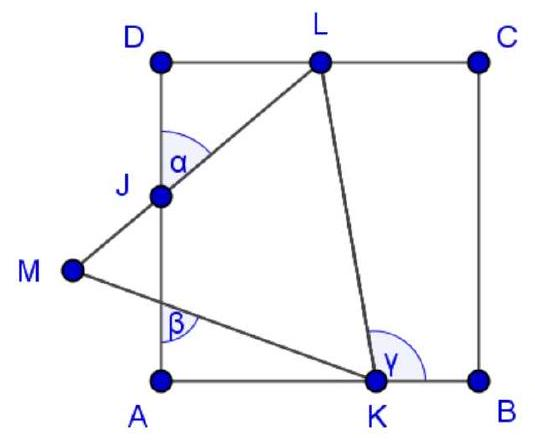
\includegraphics[max width=\textwidth, center]{2024_11_21_dcd2fc8702c4ba725104g-1}

Zadanie 5. Oblicz iloczyn: \((71-1) \cdot(71-3) \cdot(71-5) \cdot \ldots \cdot(71-97) \cdot(71-99)\).\\
\(\qquad\)

\section*{ZAŁACZNIK DO KARTY UCZESTNIKA KONKURSU „OD SZKOLNIAKA DO ŻAKA" }
Wyrażam zgodę na uczestnictwo mojego dziecka w konkursie „OD SZKOLNIAKA DO ŻAKA"

Data r.\\
(podpis rodzica lub opiekuna prawnego ucznia)

\begin{abstract}
Akceptuję i wyrażam zgodę na postanowienia regulaminu konkursu „OD SZKOLNIAKA DO ŻAKA" zamieszczonego na stronie internetowej konkursu: http:/lpg.edu.pl/kursy-z-matematyki/o-konkursie
\end{abstract}

Data r.


\end{document}